\chapter{Lorem ipsum dolor sit amet}\label{cap:exampleChapter}
% ---
\section{Aliquam vestibulum fringilla lorem}
% ---

\lipsum[1]

\begin{figure}[H]
	\begin{center}
		\label{fig:1}
		\caption{Logotipo do IFCE sem nome.}
		
\includegraphics[width=4cm]{logo-ifce-sem-nome}
		\newline
		\makebox[\width]{Fonte: Autor.}
	\end{center}
\end{figure}

% ------
\lipsum[2-3]

\includetable{tabela-exemplo} % Exemplo de inclusão de tabela

\lipsum[2-3]
% Exemplo de inclusão de gráficos
\begin{figure}
	\centering
	\caption{Exemplo de gráfico}\label{fig:animals}
	\begin{subfigure}[b]{0.45\textwidth}
		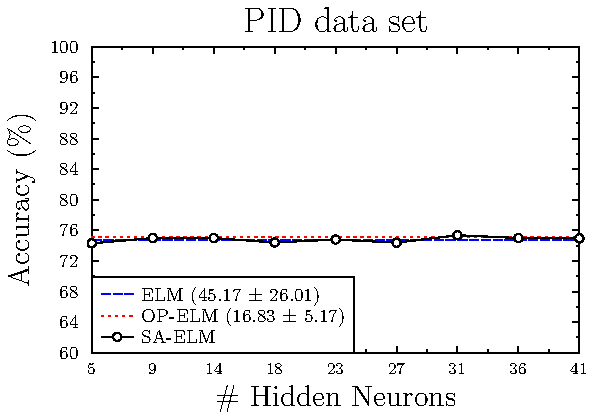
\includegraphics[width=\textwidth]{pid}
		\caption{Base de dados PID}
		\label{fig:pid}
	\end{subfigure}
	-
	\begin{subfigure}[b]{0.45\textwidth}
		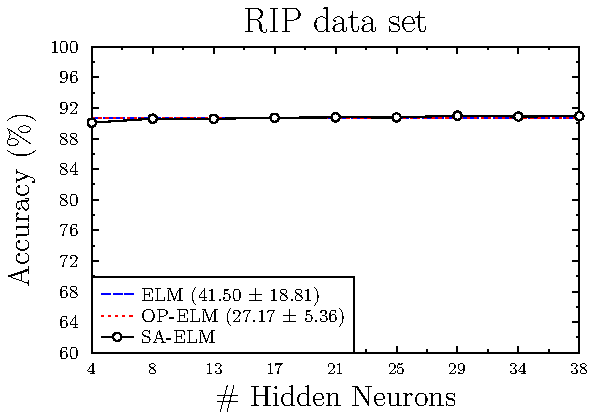
\includegraphics[width=\textwidth]{rip}
		\caption{Base de dados RIP}
		\label{fig:rip}
	\end{subfigure}
	\newline
	\makebox[\width]{Fonte: Autor.}
\end{figure}


% ------
\lipsum[2]

\begin{algorithm}
	\caption{Algoritmo de exemplo}\label{bogosort}
	\begin{algorithmic}[1]
		\Procedure{Bogosort}{array}
		\While{\Not \Call{Está\_ordenado}{array}}
		\State array $\gets$ \Call{Permutação\_aleatória}{array} \Comment{Isso vai demorar muito}
		\EndWhile
		\EndProcedure
	\end{algorithmic}
\end{algorithm}

\lipsum[1]